\subsection{Calcul du débit entrant}
Le transfert d'eau dans le réseau hydrographique est réalisé depuis les tronçons amont jusqu'à l'exutoire. A chaque nœud, les hydrogrammes amonts sont additionnés et propagés vers l’aval.

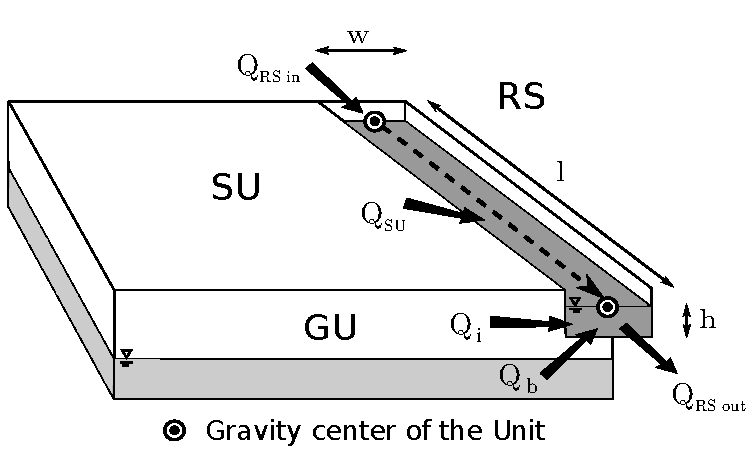
\includegraphics[width=8cm]{common/Schema_GU_RS_SU_Hayami_RS.pdf}

La première étape consiste à calculer le débit entrant dans le fossé. Il est composé du débit provenant des éventuelles unités situées en amont (RS ou SU) et des débits de subsurface et de drainage de la nappe si le modèle produit ces variables au préalable. L'équation utilisée est la suivante :

\begin{equation}
\label{InputDischarge}
Q_{in} = \sum_{RS_{Up}} Q_{RS} + \sum_{SU_{Up}} (Q_{SU} + Q_i) + \sum_{GU_{Up}} Q_b
\end{equation}


où $Q_{in}$ est le débit entrant dans le tronçon ($m\up3/s$), $Q_{RS}$ est le débit des RS amont ($m\up3/s$), $Q_{SU}$ est le débit de ruissellement des SU amont, $Q_b$ est le débit de drainage de la nappe provenant des GU ($m\up3/s$), et $Q_i$ est le débit de subsurface ($m\up3/s$).\\


\subsection{Propagation selon le noyau d'Hayami}
Ensuite, le débit entrant calculé précédemment est propagé entre l'entrée et la sortie du tronçon sur lequel est effectué le calcul. La propagation est réalisée selon le modèle de l'onde diffusante \cite{Moussa1997}, dont l'équation est la suivante :

\begin{equation}
\frac{\delta Q}{\delta t} = -C \times \frac{\delta Q}{\delta x} + D \delta \frac{\delta \up2 Q}{\delta x\up2}
\end{equation}




Dans le cas particulier où la célérité et la diffusivité de l'onde sont constantes sur le tronçon, l’équation de l’onde diffusante admet une solution analytique exacte \cite{Moussa1996}. Le débit sortant du tronçon est ainsi calculé de la façon suivante :

\begin{equation}
\label{HayamiConvolution}
Q_{RS}(t) = Q_{in}(t) * K(t)
\end{equation}




où $Q_{RS}$ est le débit produit en sortie d'unité ($m\up3/s$), $Q_{in}$ est le débit entrant dans le tronçon calculé dans l'équation \ref{InputDischarge} ($m\up3/s$), $*$ est le produit de convolution, et $K(t)$ est la fonction ``noyau d'Hayami'' qui est exprimée de la manière suivante :

\begin{equation}
K(t) = \frac{L}{2 \times (\pi D)^{\frac{1}{2}}} \times \frac{\text{exp}^{\frac{CL}{4D} \times \left(2-\frac{L}{Ct}- \frac{Ct}{L} \right) } }{t^{\frac{3}{2}}}
\end{equation}




où $L$ est la longueur du tronçon ($m$), $D$ est la diffusivité de l'onde ($m\up2/s$), et $C$ est la célérité de l'onde ($m/s$).\\

Pour réaliser la convolution de l'hydrogramme d'entrée avec l'hydrogramme unitaire d'Hayami, la fonction réalise un balayage temporel du noyau d'Hayami. $\tau$ est un opérateur de convolution avec $\delta \tau$ qui correspond au pas de temps de simulation. Cette oprétaion peut-être schématisée de la façon suivante :

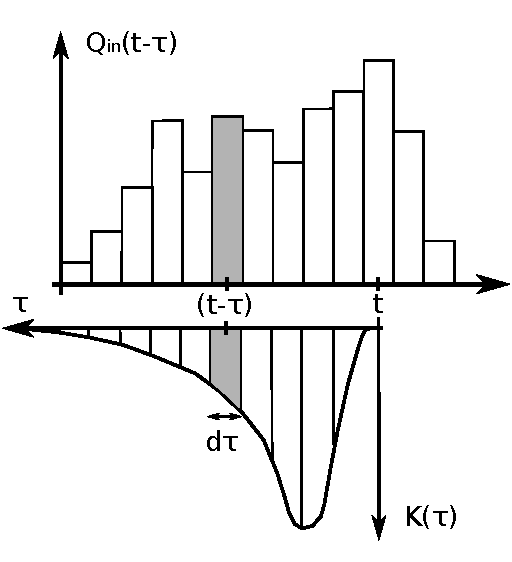
\includegraphics[width=8cm]{common/Convolution_HayamiRS.pdf}

La fonction $K(t)$ du noyau d'Hayami est défini sur le domaine [0 +$\infty$]. Cependant, la convolution ne peut être effectuée jusqu'à l'infini. On introduit alors le paramètre $MaxSteps$ ($-$) qui correspond au nombre de pas de temps maximum. La durée totale du noyau est alors égale à $MaxSteps . \Delta t$. Il doit donc être adapté en fonction de la forme du noyau d'Hayami et du pas de temps de simulation de manière à tronquer le moins possible l'hydrogramme. Plus ce paramètre sera grand, meilleure sera la définition du noyau d'Hayami. D'autre part, plus le pas de temps de simulation sera petit, meilleure sera la résolution du noyau d'Hayami.\\

Les deux paramètres $C$ et $D$ du modèle, estimés constants dans le temps, peuvent être reliés à la pente et à la rugosité du tronçon en utilisant une relation de type Manning-Strickler :

\begin{equation}
C=C_u \times \sqrt{\frac{\beta}{\beta_m}}\times \frac{n_m}{n} \ \ \ \ \ et \ \ \ \ \ D=D_u\times \frac{\beta}{\beta_m} \times \frac{n_m}{n}
\end{equation}


où $C_u$ est la célérité moyenne de l'onde ($m/s$), $\beta$ est la pente du RS sur laquelle est effectué le calcul ($m/m$), $\beta_m$ est la pente moyenne sur l'ensemble des RS ($m/m$), $n$ est le coefficient de rugosité du RS ($s/m\up{1/3}$), $n_m$ est le coefficient de rugosité moyen de l'ensemble des RS ($s/m\up{1/3}$) et $D_u$ est la diffusivité moyenne de l'onde ($m\up2/s$). Ce calcul est effectué une seule fois en début de simulation pour chaque unité.\\

La diffusivité et la célérité vont déterminer la forme de l'hydrogramme unitaire d'Hayami comme présenté sur la figure suivante :

\begin{equation}
w = \frac{L}{D} \ \ \ \ \ z = \frac{C.L}{4.D}
\end{equation}



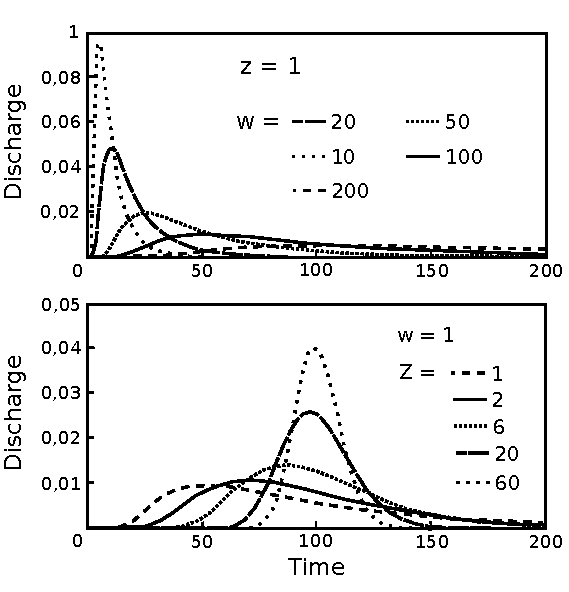
\includegraphics[width=8cm]{common/Graphique_noyau_Hayami.pdf}

Des exemples d'application et de paramétrisation de ce modèle sont disponibles dans la thèse de Chahinian \cite{Chahinian2004} et dans les travaux de Moussa et al. \cite{Moussa2002}.


\subsection{Conversion du débit en hauteur}
Le débit calculé précédemment est ensuite converti en hauteur d'eau dans le fossé. Cette transformation est réalisée grâce à l'équation de Manning-Strickler qui relie le débit à la hauteur d'eau pour une section de fossé considérée comme rectangulaire :

\begin{equation}
Q_{RS} = \frac{1}{n} \times \sqrt{\beta} \times R^\frac{2}{3} \times l \times h \ \ \ \ \text{with} \ \ \ \ R = \frac{l \times h}{l + 2h}
\end{equation}




où $n$ est le coefficient de rugosité du RS ($s/m\up{1/3}$), $\beta$ est la pente du RS ($m/m$), $R$ est le rayon hydraulique du tronçon ($m$) considéré comme ayant une section rectangulaire et dont l'expression est donnée ci-dessus, $l$ est la largeur du RS ($m$), et $h$ est la hauteur d'eau dans le tronçon ($m$) correspondant au débit.\\

La fonction calcule la courbe de calibration hauteur-débit par la relation suivante une seule fois pour chaque RS en début de simulation. Cette courbe sert ensuite à determiner, pour chaque pas de temps, la hauteur d'eau correspondant au débit calculé $Q_{RS}$. La courbe de calibration est déterminée avec un ``pas de hauteur'' donné par le paramètre $Calib Step$ (en $m$). Plus ce paramètre sera faible et plus la hauteur calculée sera précise. Cette relation est calculée jusqu'à une hauteur maximale qui est la hauteur du fossé $H$ augmentée du paramètre $RS buffer$ (en $m$). Au delà de cette hauteur, la fonction affiche un message indiquant que la hauteur d'eau dans le fossé dépasse le seuil.\\

